

%build with
%pdflatex main.tex 2>&/dev/null ; bibtex main 2>&/dev/null ; latexmk -pdf -f -g -bibtex -deps -synctex=1 -interaction=nonstopmode main.tex


%TC:macro \lstinline [xx]
%TC:envir lstlisting [] xall
\documentclass[12pt]{report}
\usepackage[paper=A4,pagesize]{typearea}
\usepackage{afterpage}
\usepackage[utf8]{inputenc}
\usepackage{graphicx}
\graphicspath{ {images/} }
\usepackage[hidelinks]{hyperref}
\usepackage[final]{pdfpages}
\usepackage{caption}
\usepackage{subcaption}
\usepackage[a4paper,width=175mm,top=25mm,bottom=25mm]{geometry}
\usepackage{fancyhdr}
\usepackage{enumitem}
\usepackage{float}
\usepackage{longtable}
\usepackage{amsmath}
\usepackage{xcolor}
\usepackage{amsmath}
\usepackage{array}
\usepackage{moreverb}
\usepackage{dirtree}
\usepackage{changepage}
\usepackage{tikz}
\usepackage[printonlyused,withpage]{acronym}
\pagestyle{fancy}
%puts chapter name in footer
\renewcommand{\chaptermark}[1]{\markboth{#1}{#1}}
\fancyhead{}
\fancyhead[R]{
Radiomics Approach to Diffusion MRI Tractography}
\fancyfoot{}
\fancyfoot[R]{\thepage}
\fancyfoot[L]{\leftmark}
\renewcommand{\headrulewidth}{0.4pt}
\renewcommand{\footrulewidth}{0.4pt}
\usepackage{titlesec}
%hides chapter text
\titleformat{\chapter}[display]{\normalfont\bfseries}{}{0pt}{\Huge}
\titlespacing*{\chapter}{0pt}{0pt}{30pt}
%paragraph indent
\setlength{\parindent}{12pt}
%paragraph spacing
\setlength{\parskip}{3pt}
%makes the numbering of the subsubsection alphabetical
\renewcommand{\thesubsubsection}{\thesubsection.\alph{subsubsection}}
\setcounter{secnumdepth}{4}
\setcounter{tocdepth}{2}
%creates left and right aligned table columns
\newcolumntype{R}[1]{>{\raggedleft\arraybackslash}p{#1}}
\newcolumntype{L}[1]{>{\raggedright\arraybackslash}p{#1}}
%code snippets
\usepackage{listings}
\usepackage{color}
\definecolor{dkgreen}{rgb}{0,0.6,0}
\definecolor{gray}{rgb}{0.5,0.5,0.5}
\definecolor{mauve}{rgb}{0.58,0,0.82}
\lstset{frame=tb,
  language=python,
  morekeywords={as},
  aboveskip=3mm,
  belowskip=3mm,
  showstringspaces=false,
  columns=fixed,
  basicstyle={\small\ttfamily},
  numbers=left,
  numberstyle=\tiny\color{gray},
  keywordstyle=\color{blue},
  commentstyle=\color{dkgreen},
  stringstyle=\color{mauve},
  breaklines=false,
  breakatwhitespace=true,
  tabsize=2
}
%references
\usepackage{csquotes}
\usepackage[utf8]{inputenc}
\usepackage[english]{babel}
\usepackage[backend=bibtex,sorting=none]{biblatex}
\addbibresource{references.bib}
%cite with clickable link wrapping some text as well
\newcommand{\citelink}[2]{\hyperlink{cite.\therefsection @#1}{#2} \cite{#1}}
%cite with clickable link wrapping some text as well
\newcommand{\reflink}[2]{\hyperref[#1]{#2} \ref{#1}}
%pdf details
\hypersetup{
  pdftitle={Enhancing Brain Connectivity Mapping: A Radiomics Approach to Diffusion MRI Tractography},
  pdfauthor={Levente Zsolt Nagy},
  pdfsubject={Medical Imaging},
  pdfkeywords={dMRI,MRI,magnetic resonance imaging,tractography,brain connectivity,radiomics,medical imaging},
  pdfcreator={Levente Zsolt Nagy},
}
%no break longtable hline
\makeatletter
\def\nobreakhline{%
  \noalign{\ifnum0=`}\fi
    \penalty\@M
    \futurelet\@let@token\LT@@nobreakhline}
\def\LT@@nobreakhline{%
  \ifx\@let@token\hline
    \global\let\@gtempa\@gobble
    \gdef\LT@sep{\penalty\@M\vskip\doublerulesep}
  \else
    \global\let\@gtempa\@empty
    \gdef\LT@sep{\penalty\@M\vskip-\arrayrulewidth}
  \fi
  \ifnum0=`{\fi}%
  \multispan\LT@cols
     \unskip\leaders\hrule\@height\arrayrulewidth\hfill\cr
  \noalign{\LT@sep}%
  \multispan\LT@cols
     \unskip\leaders\hrule\@height\arrayrulewidth\hfill\cr
  \noalign{\penalty\@M}%
  \@gtempa}
\makeatother
%title and author and date
\title{Enhancing Brain Connectivity Mapping: A Radiomics Approach to Diffusion MRI Tractography}
\author{Levente Zsolt Nagy}
\date{2024-12-15}
%word count
%actual doc
\begin{document}
%TC:ignore
\begin{titlepage}
    \begin{center}
        \begingroup
          \let\clearpage\relax

          
\includegraphics[width=1\textwidth]{banner.png}
          \vfill
          \LARGE
          \begin{center}
          \textbf{\MakeUppercase{Predicting Brain Connectivity Mapping Using Radiomics Features in Anatomical MRI}}
          \end{center}
          \vfill
          \large
          \textbf{\MakeUppercase{Levente Zsolt Nagy}}
          \vfill
          \normalsize
          \textbf{Thesis supervisor}\\
          \MakeUppercase{Alfredo Vellido Alcacena} (Department of Computer Science)\\
          \hfill\\
          \textbf{Thesis co-supervisor}\\
          \MakeUppercase{Estela Camara Mancha} (Hospital Universitari de Bellvitge)\\
          \hfill\\
          \textbf{Degree}\\
          Master's Degree in Artificial Intelligence\\
          \hfill\\\hfill\\
          \textbf{Master's thesis}\\
          \hfill\\
          \textbf{School of Engineering}\\
          \textbf{Universitat Rovira i Virgili (URV)}\\
          \hfill\\
          \textbf{Faculty of Mathematics}\\
          \textbf{Universitat de Barcelona (UB)}\\
          \hfill\\
          \textbf{Barcelona School of Informatics (FIB)}\\
          \textbf{Universitat Politècnica de Catalunya (UPC) - BarcelonaTech}\\
%           \Huge
%           \textbf{Enhancing Brain Connectivity Mapping:\\
%             A Radiomics Approach to\\
%             Diffusion MRI Tractography}

%           \vspace{0.1cm}
%           \LARGE
%           Medical Imaging

%           \vspace{1.0cm}

%           Levente Zsolt Nagy\\
%           \vspace{1.0cm}
%           \Large
%           \emph{Supervisors}\\
%           Estela Camara Mancha\\
%           Alfredo Vellido Alcacena\\
%           \LARGE

%           \vfill

%           A thesis presented for the degree of\\
%           Master in Artificial Intelligence

%           \vspace{1.0cm}
%           \includegraphics[width=0.37\textwidth]{upc.png}\\
%           \vspace{0.2cm}
%           \hspace{7px}\includegraphics[width=0.37\textwidth]{ub.png}\\
%           \vspace{0.2cm}
%           \includegraphics[width=0.37\textwidth]{bellvitge.png}\\
%           \vspace{1.0cm}

%           \Large
%           Universitat Politècnica de Catalunya\\
%           Universitat de Barcelona\\
%           Hospital Universitari de Bellvitge\\
%           Spain\\
%           2024-12-15\\
%           Number of Words: 
681
\\Number of Characters: 
3682


        \endgroup
    \end{center}
\end{titlepage}
%TC:endignore
%TC:ignore
\tableofcontents
\chapter*{List of Notations \& Abbreviations}
\begin{acronym}\itemsep0pt
  \acro{MRI}{magnetic resonance imaging}
  \acro{dMRI}{diffusion magnetic resonance imaging}
  \acro{FA}{fractional anisotropy}
  \acro{MD}{mean diffusivity}
  \acro{RD}{radial diffusivity}
  \acro{ROI}{region of interest}
  \acro{FNN}{feedforward neural network}
  \acro{FCNN}{fully convolutional neural network}
  \acro{NIfTI}{neuroimaging informatics technology initiative}
  \acro{FMRIB}{functional magnetic resonance imaging of the brain}
  \acro{FSL}{FMRIB software library}
  \acro{FNIRT}{\acs{FMRIB}'s nonlinear image registration tool}
  \acro{GLCM}{gray level co-occurrence matrix}
  \acro{GLSZM}{gray level size zone matrix}
  \acro{GLRLM}{gray level run length matrix}
  \acro{NGTDM}{neighbouring gray tone difference matrix}
  \acro{GLDM}{gray level dependence matrix}
\end{acronym}
% \listoffigures
% \listoftables
%TC:endignore

\chapter{Introduction}
\citelink{basal}{Basal ganglia is a part of the human brain which is group of subcortical nuclei responsible primarily for motor control, as well as other roles such as motor learning, executive functions and behaviors, and emotions.} \citelink{hunting}{Huntington’s disease is a disorder that causes the progressive degeneration of the basal nuclei.}\par

Hospital de Bellvitge provided an excellent dataset of \ac{MRI} and \ac{dMRI} records. This dataset contains 32 control and 37 Huntington patient records of T1 and T1/T2 \ac{MRI} images with isotropic voxels of 1 millimeter resolution and \ac{dMRI} \ac{FA}, \ac{MD} and \ac{RD} images with isotropic voxels of 2 millimeter resolution and 1 second temporal resolution. Furthermore this dataset also contains the mask for the basal ganglia, which will also be referenced as the \ac{ROI}. And taking inspiration from this \citelink{conn}{paper}, masks for the 7 main cortical regions of the brain, which will also be referenced as the target regions: Limbic, Executive, Rostral-Motor, Caudal-Motor, Parietal, Occipital and Temporal are also included in the dataset. Tractography was performed on the \ac{dMRI} images to figure out which parts of the \ac{ROI} are connected to which cortical target, in a similar manner to how it was done in said \citelink{conn}{paper}; where the relative connectivity maps are representing the ratio of the number of streamlines to each cortical target. Furthermore, the raw streamline images are also available, where there are a maximum of 5000 streamlines from each voxel in the \ac{ROI}. The anatomical segmentation of the Basal Ganglia is also available, for the Caudate Putamen and Accumbens. \par

\begin{figure}[H]
\centering
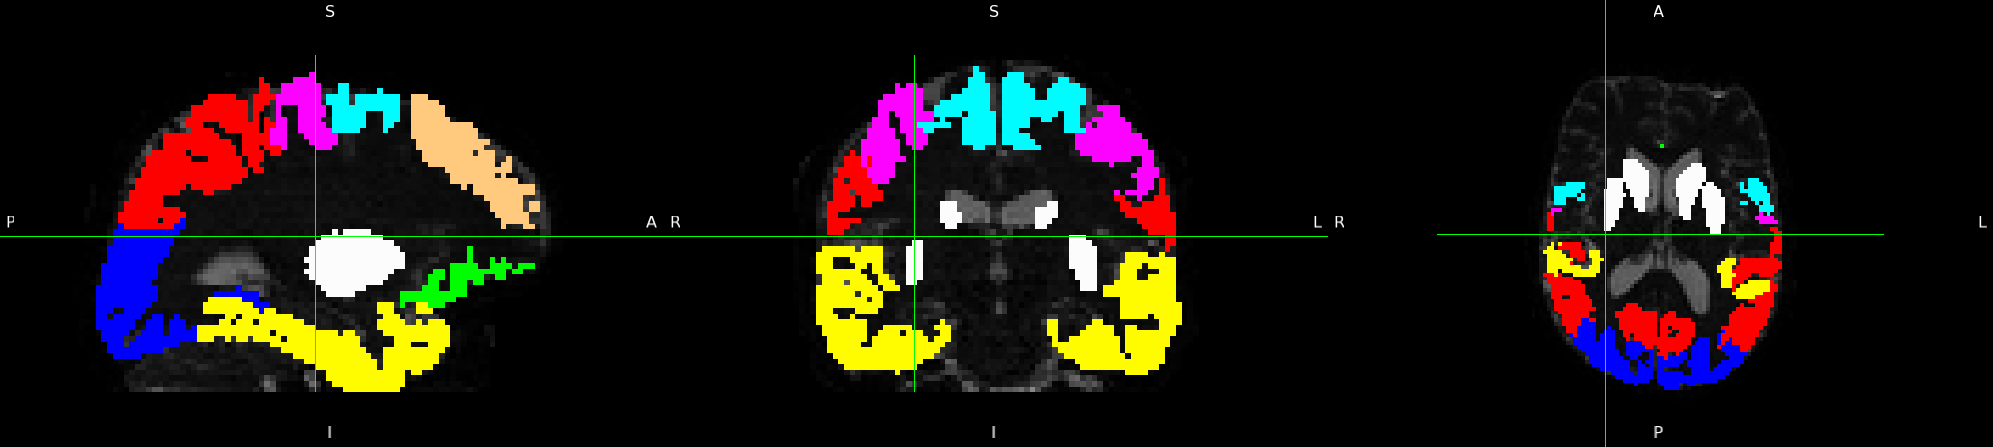
\includegraphics[width=1\textwidth]{rois}
\caption{Basal Ganglia (ROI) \& Cortical Targets}
\label{fig:rois}
\end{figure}

\begin{table}[H]
\centering
\begin{tabular}{|l|l|}
\hline
\textbf{Color} & \textbf{Region} \\ \hline
\begin{tikzpicture}\filldraw[draw=black,fill={rgb,255:red,255;green,255;blue,255}](0,0.15)rectangle(0.25,0.4);\end{tikzpicture} White & Basal Ganglia (ROI) \\ \hline
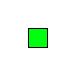
\begin{tikzpicture}\filldraw[draw=black,fill={rgb,255:red,0;green,255;blue,15}](0,0.15)rectangle(0.25,0.4);\end{tikzpicture} Green & Limbic \\ \hline
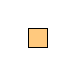
\begin{tikzpicture}\filldraw[draw=black,fill={rgb,255:red,255;green,201;blue,126}](0,0.15)rectangle(0.25,0.4);\end{tikzpicture} Brown & Executive \\ \hline

\begin{tikzpicture}\filldraw[draw=black,fill={rgb,255:red,0;green,252;blue,255}](0,0.15)rectangle(0.25,0.4);\end{tikzpicture} Light Blue & Rostral-Motor \\ \hline
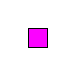
\begin{tikzpicture}\filldraw[draw=black,fill={rgb,255:red,251;green,3;blue,255}](0,0.15)rectangle(0.25,0.4);\end{tikzpicture} Purple & Caudal-Motor \\ \hline
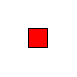
\begin{tikzpicture}\filldraw[draw=black,fill={rgb,255:red,253;green,0;blue,0}](0,0.15)rectangle(0.25,0.4);\end{tikzpicture} Red & Parietal \\ \hline

\begin{tikzpicture}\filldraw[draw=black,fill={rgb,255:red,0;green,0;blue,253}](0,0.15)rectangle(0.25,0.4);\end{tikzpicture} Blue & Occipital \\ \hline
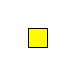
\begin{tikzpicture}\filldraw[draw=black,fill={rgb,255:red,255;green,252;blue,0}](0,0.15)rectangle(0.25,0.4);\end{tikzpicture} Yellow & Temporal \\ \hline
\end{tabular}
\caption{Regions Legend}
\label{tab:reglen}
\end{table}

Furthermore, for both the \ac{ROI} and cortical targets, the dataset distinguishes between the right and left halves of the brain. Thus there are actually 2 \ac{ROI}s and $2 \cdot 7=14$ target regions.

\begin{figure}[H]
\centering
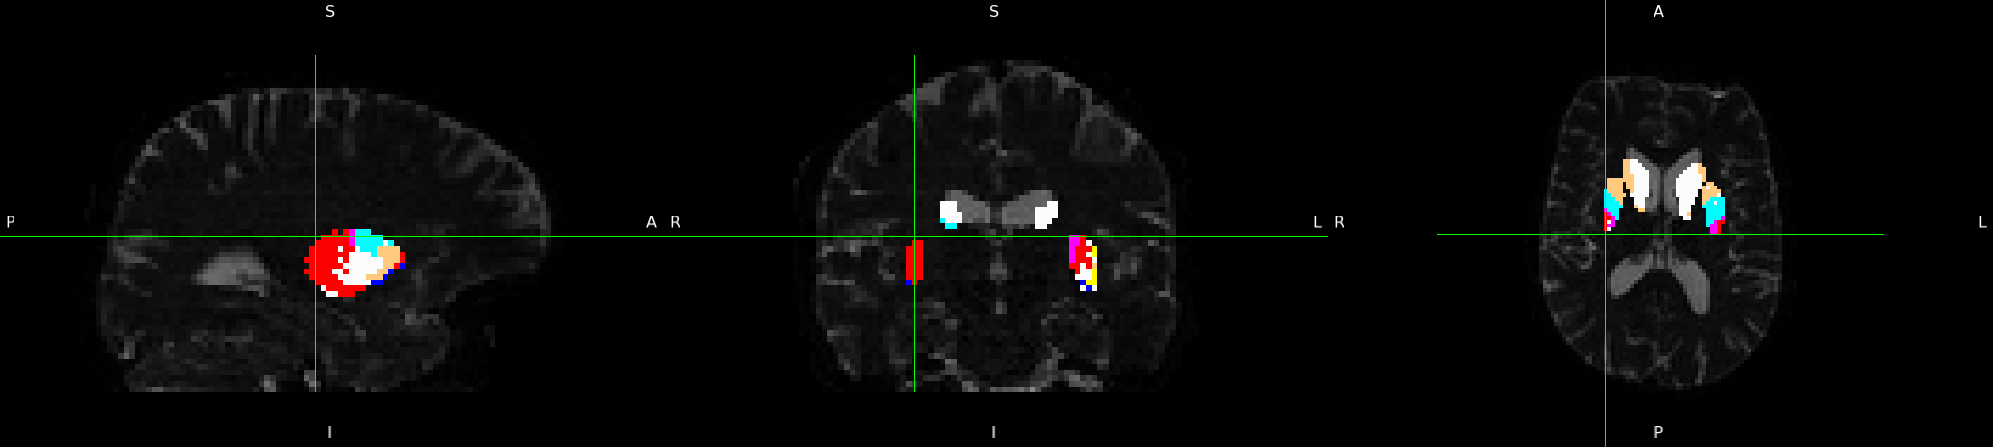
\includegraphics[width=1\textwidth]{conn}
\caption{Connectivity Maps}
\label{fig:conn}
\end{figure}

\section{Objectives}

The end goal is to predict the relative connectivity of the Basal Ganglia to the cortical targets, from the T1 and T1/T2 images.\par

This being a very complex problem, there is the possibility that the correlation between the connectivity of the brain and the T1, T1/T2 images are too weak to be mapped on this dataset. As from a datascience perspective, 69 datapoints are not much. But from a medical perspective it is substantial as it is very hard to collect uniform, clean data, with permissions to use it for research.\par

As a simpler task, leading up to the complex end goal, is a model for the simple segmentation of the Basal Ganglia for the regions Caudate Putamen and Accumbens. In order to confirm that the radiomics texture of the T1 and T1/T2 images of this dataset are are correlated to the anatomical segmentation of the Basal Ganglia. This problem is inherently connected to the main goal, as the relative connectivity does obey certain anatomical restrictions, and the anatomical segmentation of the Basal Ganglia is confirmed to be related to the relative connectivity. Thus if this simpler prediction fails, there is a good chance that the complex end goal will fail as well.\par

The biggest obstacle of this project is the preprocessing of the data, as there are many variations and hyperparameters that can be tuned. An exhaustive search definetly will not be viable, thus the preprocessing and model will needed to be tuned in a waterfall like manner, making educated guesses and comparing model performances across different tries. The main metric to measure model performance, will be the accuracy of the label prediction across voxels, as it should be comparable between all approaches.

\section{Motivation}

The motivation for predicting the connectivity maps from the T1 and T1/T2 \ac{MRI} images, is skipping the time and resource consuming process performing \ac{dMRI} and tractorgrapy.

\section{State of the Art}

Me :)




























\chapter{Fulfillment of the Objectives}
\section{Objectives}

The end goal is to predict the relative connectivity of the Basal Ganglia to the cortical targets, from the radiomics features of the T1 and T1/T2 images.\par

This being a very complex problem, there is the possibility that the correlation between the connectivity of the brain and the T1, T1/T2 images are too weak to be mapped on this dataset. As from a datascience perspective, 69 datapoints are not much. But from a medical perspective it is substantial as it is very hard to collect uniform, clean data, with permissions to use it for research.\par

A simpler task leading up to the complex end goal, is a model for the simple segmentation of the Basal Ganglia for the subcortical regions Caudate, Putamen and Accumbens. In order to confirm that the radiomics texture of the T1 and T1/T2 images of this dataset are are correlated to the segmentation of the Basal Ganglia. This problem is inherently connected to the main goal, as the relative connectivity does obey certain anatomical restrictions, and the subcortical segmentation of the Basal Ganglia is confirmed to be related to the relative connectivity. Thus if this simpler prediction fails, there is a good chance that the complex end goal will fail as well.\par

Another intermediate task, is a model for predicting \ac{FA} and \ac{MD} images. This is also related to the main goal, as these images are computed from the \ac{dMRI} images, the same image that the relative connectivity was computed from. But it is inherently simpler, not needing to perform complex algorithms like tractography.\par

The biggest obstacle of this project is the preprocessing of the data, as there are many variations and hyperparameters that can be tuned. An exhaustive search definitely will not be viable, thus the preprocessing and model will needed to be tuned in a waterfall like manner, making educated guesses and comparing model performances across different tries. The main metric to measure model performance, will be the accuracy of the label prediction across voxels, as it should be comparable between all approaches. The accuracy metric will be used for the subcortical label prediction problem as well, and pearson correlation will be used as the metric to evaluate the \ac{FA} and \ac{MD} predictions.

\section{Motivation}

The motivation for predicting the connectivity maps from the T1 and T1/T2 \ac{MRI} images, is skipping the time and resource consuming process performing \ac{dMRI} and tractorgraphy.

\section{Experiments}

The following contributing factors are needed to be explored and experimented with:
\begin{itemize}
  \item Experiment Type:
  \begin{itemize}
    \item Basal Ganglia subcortical segmentation (classification)
    \item Brain / Basal Ganglia diffusion \ac{FA} and \ac{MD} prediction (regression)
    \item Basal Ganglia relative connectivity segmentation (classification)
    \item Basal Ganglia number of streamlines prediction (regression)
  \end{itemize}
  \item Input Space:
  \begin{itemize}
    \item Native
    \item Normalized
  \end{itemize}
  \item Input Data:
  \begin{itemize}
    \item T1
    \item T1/T2
    \item Mixed (T1 and T1/T2)
  \end{itemize}
  \item Radiomics Extraction Parameters:
  \begin{itemize}
    \item Kernel size
    \item Bin width
    \item Relative bin width (fixed number of bins)
  \end{itemize}
  \item Additional Non-Voxel Based Radiomics Inputs:
  \begin{itemize}
    \item Basal Ganglia
    \item Entire Brain
    \item Target Regions
  \end{itemize}
  \item Left and Right Hemispheres:
  \begin{itemize}
    \item Left only
    \item Right only
    \item Left and Right with concatenated label information (e.g. no differentiation between left and right target regions)
    \item Left and Right with NOT concatenated label information (e.g. differentiation between left and right target regions)
  \end{itemize}
  \item Control and Patient Datapoints:
  \begin{itemize}
    \item Control only
    \item Patient only
    \item Mixed (Control and Patient)
  \end{itemize}
  \item Additional Clinical Data Input
  \item Sequential Backward Feature Selection
  \item Feature Scaling and/or Normalization
  \item Relative Connectivity Thresholding
  \item Model Properties
  \begin{itemize}
    \item General Architecture
    \begin{itemize}
      \item Single FNN Model
      \item Dual FNN Model (more on this later)
      \item Mixture of Experts FNN Model (more on this later)
    \end{itemize}
    \item Model Size
    \begin{itemize}
      \item Number of Layers
      \item Layer Width
    \end{itemize}
    \item Activation Function
    \item Batch Size
    \item Early Stopping
    \item Loss Function
    \item Learning Rate
    \item Regularization
  \end{itemize}
\end{itemize}

As mentioned, an exhaustive search of the hyperparameter space is not feasible, thus it must be explored in a linear way. The following experiments are already done, or partially done:

\begin{itemize}
  \item Basal Ganglia subcortical segmentation
  \begin{itemize}
    \item Sanity Check: tried to predict it from T1 to make sure there is no direct correlation
    \item Additional Non-Voxel Based Radiomics Inputs: experimented with additional non-voxel based radiomics features
    \item Radiomics Kernel Sizes: experimented with including voxel based features with different kernel sizes
    \item Short Conclusion: including multiple different kernel sizes are the best, non-voxel based features made no improvement, final test accuracy 0.91
  \end{itemize}
  \item Brain / Basal Ganglia diffusion \ac{FA} and \ac{MD} prediction
  \begin{itemize}
    \item \ac{FA}: predicted \ac{FA} in Basal Ganglia from many different kernel sizes (did not use any other features besides voxel based radiomics), yielded test pearson correlation of 0.92
    \item \ac{MD}: predicted \ac{MD} in Basal Ganglia from many different kernel sizes (did not use any other features besides voxel based radiomics), yielded test pearson correlation of 0.83
  \end{itemize}
\end{itemize}

After completing the two simpler exercises, and confirming the viability of the thesis, I moved onto the relative connectivity prediction. I ran experiments for the following 6 configurations:

\begin{itemize}
  \item T1 native space
  \item T1/T2 native space
  \item T1 native space (excluding datapoints that are missing T1/T2 for fair comparison)
  \item T1 normalized space
  \item T1/T2 normalized space
  \item T1 normalized space (excluding datapoints that are missing T1/T2 for fair comparison)
\end{itemize}

Experiments:

\begin{itemize}
  \item Single kernel size voxel based features
  \begin{itemize}
    \item Additional non-voxel based features of target regions (single bin)
    \item Additional non-voxel based features of basal ganglia (single bin)
    \item Additional non-voxel based features of basal ganglia \& whole brain (single bin)
  \end{itemize}
  \item 4 different kernel sized voxel based features \& 4 different bin sized basal ganglia features
  \item 2 different kernel sized voxel based features \& 2 different bin sized basal ganglia features
  \item 5 different kernel sized voxel based features \& single bin size basal ganglia features
  \item 4 different kernel sized voxel based features
  \item 9 different kernel sized voxel based features
  \begin{itemize}
    \item control datapoints
    \begin{itemize}
      \item left hemisphere
      \item right hemisphere
      \item both hemisphere
    \end{itemize}
    \item huntington datapoints
    \begin{itemize}
      \item left hemisphere
      \item right hemisphere
      \item both hemisphere
      \begin{itemize}
        \item included CAP clinical data
        \item included CAP \& UHRDs clinical data
        \item included all clinical data
      \end{itemize}
    \end{itemize}
    \item both control \& huntington datapoints
    \begin{itemize}
      \item left hemisphere
      \item right hemisphere
      \item both hemisphere
    \end{itemize}
  \end{itemize}
\end{itemize}

Tried two different model configurations, a simple FNN for classifying datapoints. And a dual model FNN, where one of them predicts the connectivity label and the other one is a regression model responsible for predicting the connectivity value of the strongest connection. The latter one can be used to 'reinforce' the not connected voxels, achieving a better accuracy. The best performing configuration so far was Native T1/T2, with all 9 voxel based features (without non-voxel based features), on control datapoints, with both left and right hemispheres included, yielding 0.62 accuarcy on the test datapoints. Some preliminary observations are:

\begin{itemize}
  \item Right hemisphere datapoints are consistently easier to predict that left datapoints
  \item Control datapoints are consistently easier to predict that huntington datapoints
  \item Combining control and huntington datapoints inconsistently yielded same, or marginally better accuracy
  \item Combining right and left hemisphere datapoints inconsistently yielded same, or marginally better accuracy
  \item Including clinical data for the huntington datapoints resulted in less overfitting and better accuracy (BUT still worse than control datapoints)
  \item Multiple, larger kernel sizes are better (still experimenting what is the best)
  \item T1/T2 is better
  \item Including target region features resulted in less overfitting, and marginally worse accuracy
  \item Including basal ganglia features resulted in more overfitting, and worse accuracy
  \item Including basal ganglia and brain features resulted in more overfitting, and worse accuracy
  \item Dual FNN model (for not connected reinforcement) consistently yielded much better accuracy
\end{itemize}







\chapter{Adjustments Made}

The main adjustment was changing the focus of the main goal of predicting relative connectivity, to predicting \ac{FA} and \ac{MD}. Due to the yielded results being underwhelming, regardless that with further fine tuning we could get the accuracy up to maybe around 0.7 which is much-much better than random guessing. And the \ac{FA} and \ac{MD} predictions look more promising and easier to work with, so we want to focus the remaining resources on fine tuning and experimenting with those models.\par

Other deviations from the original plans, is that we are not even going to try using a highly explainable model (such as decision trees), as it is evident at this point that the complexity of this problem is beyond the capabilities of said models. Furthermore we will not try fully convolutional approaches, after realizing that it does not fit the original hypothesis of 'can we predict relative connectivity from the radiomic features'. As well as other technical limitations, as a simple U-net with 3 downasmple and 3 upsample layers, were already huge enough so it would only work with a maximum batch size of 1, on a GPU with 24GBs of VRAM.\par

And lastly we would like to change the title of the thesis to 'Brain Connectivity Mapping with Structural MRI' \textcolor{red}{(waiting for a final confirmation from Estela)} from 'Characterizing Neurodegeneration Patterns Using Radiomics' as it did not completely fit for what we are trying to do.
\chapter{Work Plan for Completion}
The remaining time and resources will be focused on completing the following tasks:

\begin{itemize}
  \item Refine Train/Validation/Test splitting, as of right now it is not ensured that the splits contain the same ratio of asymptomatic and symptomatic huntington patients (it has been pointed out to me that asymptomatic patients' neurodegeneration is very similar to controls' meaning it can skew the results).
  \item Refine normalized space evaluation, as of right not it is not a completely fair comparison between native and normalized space. A solution will be implemented to 'de-normalize' the yielded predictions into native space, and compute the final metric in the native space, resulting in a more fair comparison.
  \item More detailed and in-depth experimentation for \ac{FA} and \ac{MD} predictions (similar to the relative connectivity experimentations).
  \item Finishing exhaustive feature selection on the relative connectivity (it is computationally expensive and it is half way done, and hopefully it can be used for FA and MD as well).
  \item One unorthodox idea that is yet to be tried is to append the coordinates of each voxel to the normalized input space. As the model could learn anatomical markers based on this.
  \begin{itemize}
    \item An extension of this idea is to include the coordinates in native space as well. This by default would not make sense as the coordinates of voxels between different patients are not comparable in native space. But first extracting the coordinates in normalized space and then warping them back to native space by 'de-normalizing' them, could work.
  \end{itemize}
  \item Fine tuning the best model for predicting voxels separately for each spaital location. This approach capitalizes on the same idea as including the voxel coordinates, as the fine tuned models could learn extra anatomical markers based on their spatial locations. (similarly, this only makes sense in normalized space)
\end{itemize}


%TC:ignore
% \printbibliography[heading=bibintoc,title={Sources of Information}]

%================== EXAMPLES ==================
% \includepdf[pages=1,pagecommand={\chapter[Project Description]{} \label{app:projdesc}},linktodoc=true]{Appendix_A/ProjectDescription.pdf}
% \includepdf[pages=2-]{Appendix_A/ProjectDescription.pdf}
% \chapter{Machine Vision Class Descriptions} \label{app:CVclassdesc}
% \input{appendices/classdesccpp}
% \chapter{Source Code} \label{app:sourcecode}
% \label{apx:source}

\dirtree{%
.1 source.
.2 data.
.3 models.
.3 native.
.4 preloaded.
.4 preprocessed.
.4 raw.
.3 normalized.
.4 preloaded.
.4 preprocessed.
.4 raw.
.3 preprocessed.
.3 raw.
.2 logs.
.2 fsleyes.
.2 distributed.
.1 experiments.
.2 subcortical.
.2 diffusion\_md.
.3 native-t1.
.3 native-t1t2.
.3 normalized-t1.
.3 normalized-t1t2.
.3 architecture.
.2 diffusion\_fa.
.3 native-t1.
.3 native-t1t2.
.3 normalized-t1.
.3 normalized-t1t2.
.3 architecture.
.2 connection.
.3 native-t1.
.3 native-t1t2.
.3 normalized-t1.
.3 normalized-t1t2.
.3 architecture.
.2 streamline.
.2 misc.
.1 report.
.2 progress.
.2 project.
}


% \texttt{ }\par
% \noindent \textbf{android-camera-imu} the source code of the auxiliary camera-imu app\par
% \texttt{ }\par
% \noindent \textbf{diagrams} exported UML diagrams\par
% \texttt{ }\par
% \noindent \textbf{doc} some of the \path{.tex} files\par
% \noindent \textbf{appendices} appendix \path{.tex} files\par
% \noindent \textbf{chapters} chapter \path{.tex} files\par
% \noindent \textbf{images} figures\par
% \includepdf[pages=1,pagecommand={\chapter[User Manual]{} \label{app:manual}},linktodoc=true]{Appendix_D/UserManual.pdf}
% \includepdf[pages=2-]{Appendix_D/UserManual.pdf}
% \chapter{Unit Test Descriptions and Test Results} \label{app:CVunittestdesc}
% \input{appendices/unittestdesccpp}
% \chapter{Integration Test Results} \label{app:CVintegrationtestdesc}
% \input{appendices/integrationtestdesccpp}
% \includepdf[pages=1,pagecommand={\chapter[Process Report]{} \label{app:procrep}},linktodoc=true]{Appendix_G/ProcessReport.pdf}
% \includepdf[pages=2-]{Appendix_G/ProcessReport.pdf}
%==============================================

%TC:endignore
\end{document}